
%(BEGIN_QUESTION)
% Copyright 2008, Tony R. Kuphaldt, released under the Creative Commons Attribution License (v 1.0)
% This means you may do almost anything with this work of mine, so long as you give me proper credit

Identify the state of the light bulb when the normally-closed pressure switch contact {\it opens}:

$$\includegraphics[width=15.5cm]{i03204x01.eps}$$

Assuming the light bulb functions as a pressure alarm to alert operators to an unsafe condition, determine whether this is a {\it low-pressure} alarm or a {\it high pressure} alarm.

\vskip 10pt

Hint: remember that the ``normal'' status of a switch is defined as the status of {\it minimum stimulus}: when the switch is exposed to the lowest possible degree of process stimulation (in this particular case, to the lowest possible pressure).

\underbar{file i03204}
%(END_QUESTION)





%(BEGIN_ANSWER)

When the pressure switch contact opens, the relay de-energizes, closing the normally-closed relay contact and turning the light on.

\vskip 10pt

This circuit functions as a {\it high-pressure} alarm, turning the light bulb on if the process pressure ever rises above switch's trip value.
 
%(END_ANSWER)





%(BEGIN_NOTES)


\filbreak \vskip 20pt \vbox{\hrule \hbox{\strut \vrule{} {\bf Virtual Troubleshooting} \vrule} \hrule}

\noindent
{\bf Predicting the effect of a given fault:} present each of the following faults to the students, one at a time, having them comment on all the effects each fault would produce.

\begin{itemize}
\item{} 
\item{} 
\item{} 
\end{itemize}


\vskip 10pt


\noindent
{\bf Identifying possible/impossible faults:} present symptoms to the students and then have them determine whether or not a series of suggested faults could account for all the symptoms, explaining {\it why} or {\it why not} for each proposed fault:

\begin{itemize}
\item{} Symptom: {\it }
\item{}  -- {\bf Yes/No}
\item{}  -- {\bf Yes/No}
\item{}  -- {\bf Yes/No}
\end{itemize}


\vskip 10pt


\noindent
{\bf Determining the utility of given diagnostic tests:} present symptoms to the students and then propose the following diagnostic tests one by one.  Students rate the value of each test, determining whether or not it would give useful information (i.e. tell us something we don't already know).  Students determine what different results for each test would indicate about the fault, if anything:

\begin{itemize}
\item{} Symptom: {\it }
\item{}  -- {\bf Yes/No}
\item{}  -- {\bf Yes/No}
\end{itemize}


\vskip 10pt


\noindent
{\bf Diagnosing a fault based on given symptoms:} imagine the wire connecting the NC terminal of the switch to the relay coil fails open in this system (don't reveal the fault to students!).  Present the operator's observation(s) to the students, have them consider possible faults and diagnostic strategies, and then tell them the results of tests they propose based on the following symptoms, until they have properly identified the nature and location of the fault:

\begin{itemize}
\item{} {\it Lamp is always on, regardless of fluid pressure}
\item{} $V_{2-7}$ (relay coil) = 0 volts at all times
\item{} $V_{1-4}$ (relay NC contacts) = 0 volts at all times
\item{} $V_{Com-NC}$ (switch) = 0 volts at all times
\end{itemize}

%INDEX% Pictorial circuit review (relay circuit)

%(END_NOTES)


